%---------------------------------------------------------------
%	UNIVERSIDADE FEDERAL DE UBERLÂNDIA
%	Faculdade de Engenharia Elétrica
%	Programa de Pós-Graduação em Engenharia Elétrica
%	Programa de Pós-Graduação em Engenharia Biomédica
%	Laboratório de Engenharia Biomédica
%	Dissertação de Mestrado
%	Capítulo 1: Introdução
%---------------------------------------------------------------
\section{Introdução}
\label{cap4:introducao}
Uma máquina síncrona, em condições de regime permanente, é uma máquina CA cuja velocidade é proporcional à frequência da corrente de sua armadura. O rotor, juntamente com o campo magnético criado pela corrente CC do campo do rotor, gira na mesma velocidade ou em sincronismo com o campo magnético girante, produzido pelas correntes de armadura, resultando um conjugado constante.
%

Um gerador síncrono é composto por uma parte fixa (estator) e uma parte rotativa (rotor). Emprega-se material magnético nas duas estruturas para guiar o fluxo magnético e enrolamentos são utilizados para conduzir corrente elétrica. Uma estrutura composto por um par de pólos é apresentada na figura \ref{maq_sinc}.
%
\begin{figure}[H]
\centering
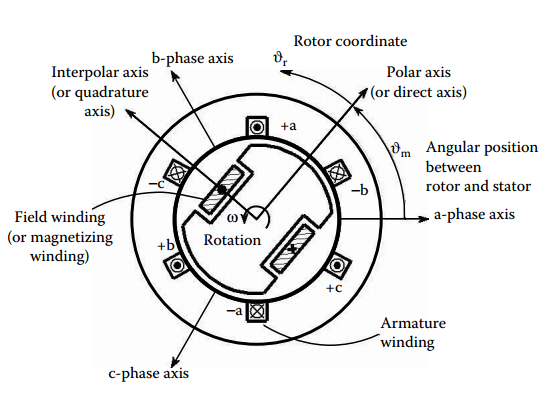
\includegraphics[scale=0.9]{img/assig4/ger_sinc_3ph.png}
\caption[Estruturas e referências de um gerador síncrono trifásico]{Estruturas e referências de um gerador síncrono trifásico. Extraído de \cite{Bianc}.}
\label{maq_sinc}
\end{figure}
